\chapter{Nature of Nuclear Force}

    \begin{tcolorbox} [colframe=blue!10!black,colback=yellow!29.05!white,arc=1em,fonttitle=\bfseries,title= Key Objectives:, width = \textwidth]
        $\star$ \textbf{Origin of Nuclear Force} $\star$
        \begin{itemize}
            \item Strong Interaction(You may go through \\ \nameref{chap:funda})
        \end{itemize}
       $\star$ \textbf{Properties of Nuclear Force} $\star$ 
       \begin{itemize}
             \item Range (based on existing knowledge of Binding Energies) 
                \begin{itemize}
                    \item Short Range: Saturation Property
                    \item Repulsive Core: Concept of Incompressibility and Uniform Density of Nuclear Matter
                \end{itemize}
             \item Charge Independence and Charge Symmetric (Isospin)
       \end{itemize}
     \end{tcolorbox}
     
 \pagebreak   \section{Origin of Nuclear Charge}
            \begin{figure}
                \centering
                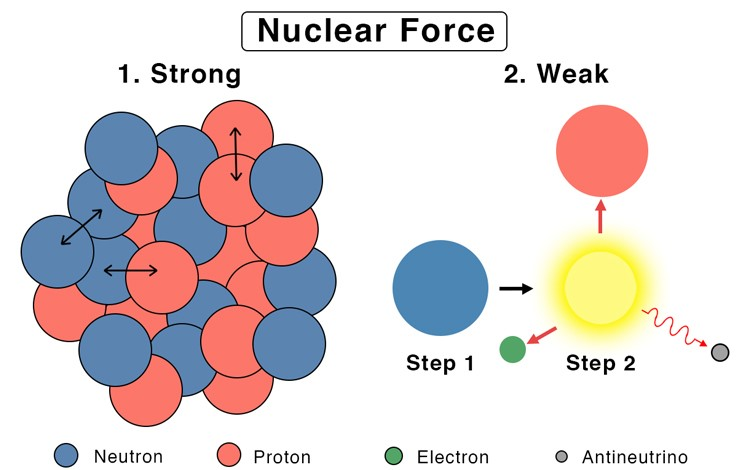
\includegraphics[width = 0.75\textwidth]{01/IMG4.jpg}
            \end{figure}
  The nuclear force (or nucleon–nucleon interaction) is a force that acts between the protons and neutrons and holds them inside the nucleus. In this class, we only need to know that the nuclear force is a residual effect of a fundamental force, namely the \href{https://en.wikipedia.org/wiki/Strong_interaction}{Strong interaction}. The Strong interaction binds the elementary particles known as \href{https://en.wikipedia.org/wiki/Quark}{quarks} which form the protons and neutrons.
      It is really fascinating how neutrons and protons are packed inside the tiny space \textit{(~few fm)} of a nucleus. Moreover, protons are positively charged and, hence, they must feel the tremendous repulsion due to Coulomb force. Thus, the nuclear force must be more powerful than the electromagnetic interaction (Coulomb interaction). However, in order to get more fundamental insight to our question of the nature of the nuclear force, we need to know a few basic things about the fundamental interactions in nature. Therefore, I request you to read the chapter \nameref{chap:funda}, if you are keen to know the underlying physics.\textit{ However, you may skip it for the time being and it will cause no harm to learn nuclear physics in its low energy domain. }

\section{Properties of Nuclear Force}
        $\bullet$~\textbf{Range:} Nuclear force is short range in nature and more powerful than the electromagnetic interaction. The nuclear force is extremely attractive between the nucleons at distances of about 1 fm. However, it decreases sharply beyond that and becomes insignificant beyond $\sim$ 2.5 fm. Due to this short range, a nucleon inside a nucleus can only interact with a few nucleons in its vicinity. This is known as the \textbf{Saturation property} of the nuclear force. Obviously, it must have come to your mind, how short is this ``Short range means"? This can be measured experimentally and even theoretically.
        
        \begin{wrapfigure}{r}{0.5\textwidth}
        %\centering
        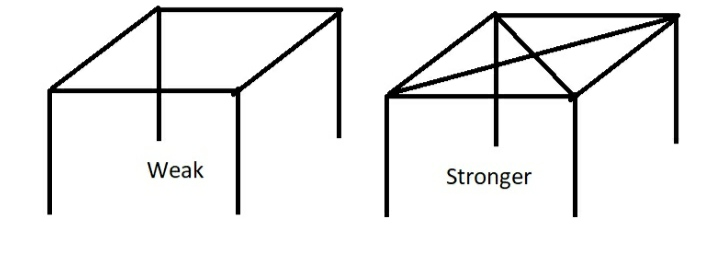
\includegraphics[width=0.5\textwidth]{01/IMG0.jpg}
        %\caption{\\Proton-neutron interaction}
        %\label{fig:nucleons}
        \end{wrapfigure}
        
$\star$~{\textbf{Read the following to have a better understanding of the short range nature of Nuclear Force: }}
\par Suppose you are building a house with bamboo sticks., you must have placed only four corner posts and connect them with one stick between each corner. At this time, your structure is not that strong. But as you keep on adding more and more connections (bamboos) between them, they become stronger and stronger. If you agree then let us analyse a nucleus.
 \par Replace the corners with nucleons (protons or neutrons) and the bamboos with the nuclear force.\textbf{ This model states that if we allow each nucleon inside a nucleus to interact with all the other nucleons inside it} then the heavier the nucleus, stronger the binding for each nucleon (imagine your Bamboo model).
         \begin{wrapfigure}{l}{0.5\textwidth}
        %\centering
        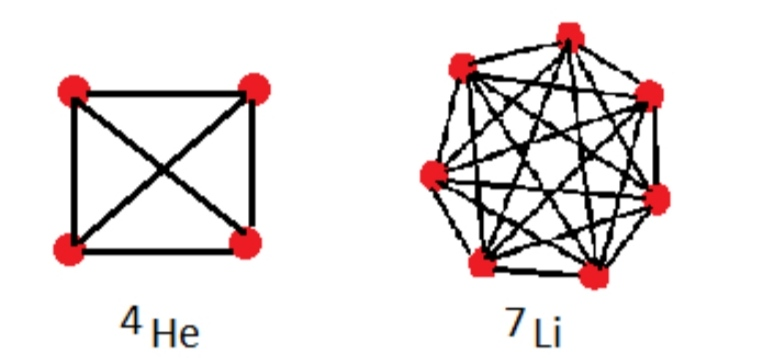
\includegraphics[width=0.5\textwidth]{01/IMG1.jpg}
        %\caption{\\Proton-neutron interaction}
        %\label{fig:nucleons}
        \end{wrapfigure}
Let us look at an example. In $^{4}He$, each nucleon has 3 connections and in $^{7}Li$ each nucleon has 6 connections. Thus, each nucleon in  $^{7}Li$ must be more strongly bounded than $^{4}He$. Similarly in $^{235}U$, there are 234 connections! Thus, B.E./A in $^{235}U$ should have been strongest. This can also be shown mathematically. If we consider the above assumption then a nucleus with A number of nucleons, can interact with A-1 other nucleons. So the total binding energy (B.E.) is proportional A(A-1)/2 (2 in the denominator to compensate for the double counting of the same pair of nucleons). If A is large, we may consider the B.E. is proportional $A^2$. Hence, B.E./A is proportional to A and B.E./A plot would be a monotonically increasing straight line graph. But, this is not what we have learnt from the B.E./A plot (B.E./A is nearly constant and it is around 8 MeV).

The above analysis tells us that nuclear force is  short range. Therefore, a nucleon can only interact with a few nearby nucleons. Therefore, B.E. is not proportional to A.(A-1) but proportional to A. Hence, B.E./A is constant which is a direct consequence of the short range nature of the nuclear force. 

        $\bullet$~\textbf{Hard Core:} In order to prevent the nucleus from collapsing from the tremenduous powerful attraction, a repulsive component exists in the nuclear force. This short-range repulsive force becomes very large and repulsive for separations less than about 0.7 fm.
        \begin{wrapfigure}{r}{0.5\textwidth}
        %\centering
        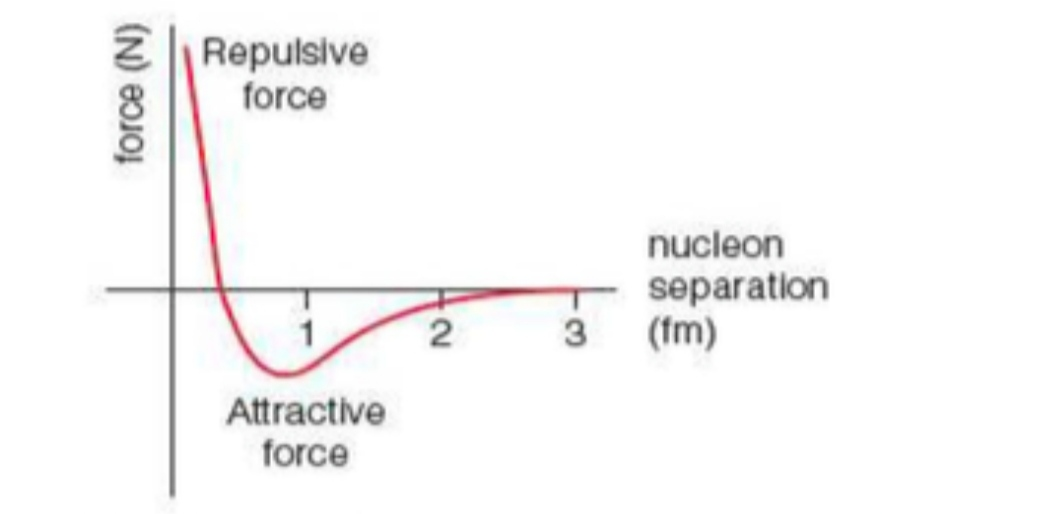
\includegraphics[width=0.5\textwidth]{01/IMG2.jpg}
        %\caption{\\Proton-neutron interaction}
        %\label{fig:nucleons}
        \end{wrapfigure}
        The adjacent figure shows the results of the superposition of the short range attractive and the repulsive force components. Thus, it maintains the similar average separation between the nucleons in all nuclei.\textbf{ It leads to the uniform density of nuclear matter ($\sim~2.3×10^{17}$ kg/m3) and will be used to calculate the radius of a nucleus.}   
        
        $\bullet$~\textbf{Charge Symmetric \& Charge Independence:} Experiments show that Nuclear Force is not affected bu Coulomb interaction. Therfore, it is the same between two protons or neutrons inside a nucleus. Of course, the Coulomb repulsion has not been taken into account. This is known as charge symmetry of nuclear force and symbolically:
        \begin{equation}
            (n-n)~=~(p-p)
        \end{equation}
Thus,  the force between a proton and neutron should be the same as the above. Hence,
        \begin{equation}
            (n-n)~=~(p-p)~=~(p-n)
        \end{equation}
 
         \begin{wrapfigure}{l}{0.55\textwidth}
        %\centering
        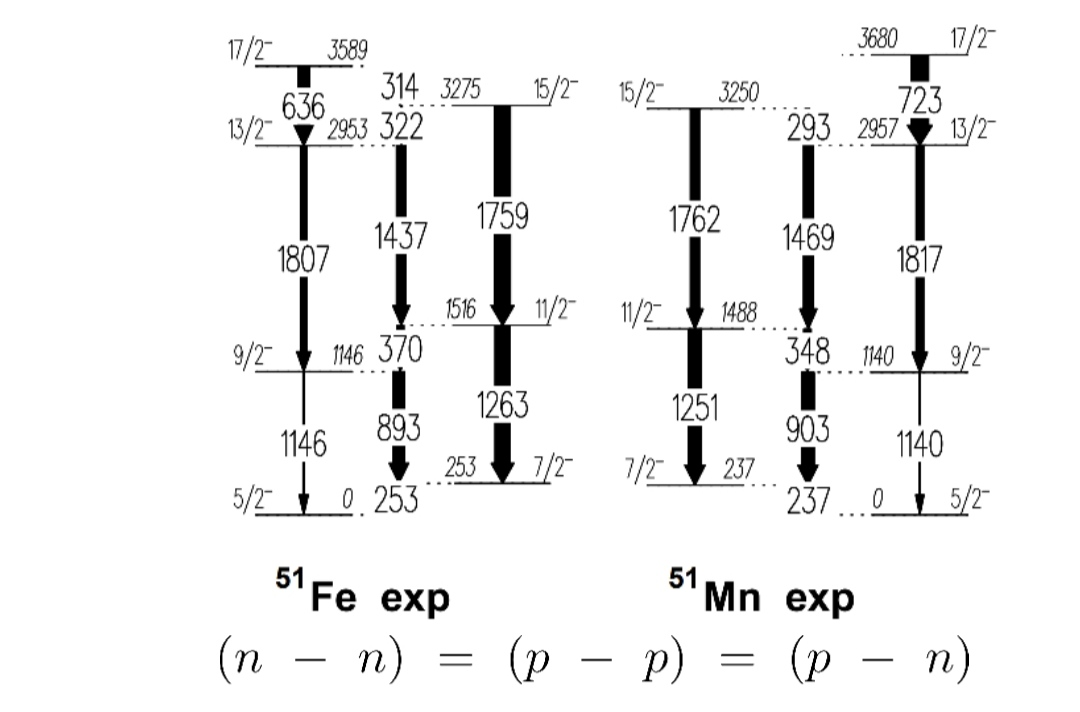
\includegraphics[width=0.55\textwidth]{01/IMG3.jpg}
        %\caption{\\Proton-neutron interaction}
        %\label{fig:nucleons}
        \end{wrapfigure}
This is called charge independence. Thus, inside a nucleus, the charge symmetry is broken by the electromagnetic interaction due to the charge of the proton. The validity of this hypothesis is substantiated with the striking similarity in the excitation spectra of \href{https://en.wikipedia.org/wiki/Mirror_nuclei}{mirror nuclei} and in the n-n, n-p and p-p scattering experiments.


\par$\bullet$~\textbf{Isospin:} Based on the above concept a hypothesis was introduced (before the quark came into the picture) where proton and neutron are considered as two different states of a nucleon. The nucleon-nucleon force is the same irrespective of whether the nucleons are protons or neutrons - once the coulomb repulsion has been taken out. Hence, we can introduce a new quantum number, Isospin, similar to that of electron spin (S), to define two states, one for protons and the other for neutrons. We assign an isospin value of 
\begin{equation}
   \tau = 1/2
\end{equation}(in the same way, as we assign   for S = 1/2 electron spin). In low-energy nuclear physics, we chose the isospin projection
\begin{equation}
   \tau_z = 1/2
\end{equation}
for neutrons and
\begin{equation}
\tau_z = -1/2
\end{equation}
for protons  which are opposite in particle physics.  

    
\par\textbf{\underline{Note:}} \textit{It is to be noted that even after almost 100 years of our best efforts, understanding of the nuclear potential is still incomplete. The primary problem is that the experimental data suggest that there is a three body interaction component in the nucleon-nucleon interaction. Such interaction among a finite number of particles requires advanced mathematical techniques and moreover computational support to handle such large scale calculation. This is a front-end research domain and till date successful for nuclei up to  $A=12$.}      
      